\chapter{Mètodes pertorbatius i modes acoblats}

\section{Introducció}

Encara que podem resoldre problemes molt complexos mitjançant càlcul numèric, ens interessa obtindre solucions analítiques, encara que siguen aproximades, per a alguns casos. Als ressonadors, per exemple, podem calcular les freqüències de ressonància, però si fem un forat per introduir els camps canviem les condicions de contorn i, molt probablement, deixem de tindre solució analítica. Igualment, quan dues línies dielèctriques s' apropen massa els modes s' acoblen i deixem de tindre solucions. Aquests són dos exemples de situacions que, com vorem, podem resoldre usant mètodes pertorbatius i teoria de modes acoblats, respectivament.

\section{Mètodes pertorbatius}

Els mètodes pertorbatius ens permeten calcular, a partir dels camps electromagnètics d' un sistema, els camps d' un sistema idèntic al primer excepte per xicotetes diferències anomenades pertorbacions. Hi ha dos tipus principals de pertorbacions: pertorbacions de forma i pertorbacions del material.

\subsection{Pertorbacions materials}

Tenim un sistema ressonant del que coneixem les $\omega _0$, i volem trobar les noves $\omega _0$ en cas de que fem un xicotet canvi $\epsilon \to \epsilon + \Delta \epsilon$ i $\mu \to \mu + \Delta \mu$ a les propietats del material (figura \cref{perturbmaterial}). Els camps originals satisfan:

\begin{figure}[ht]
  \centering
  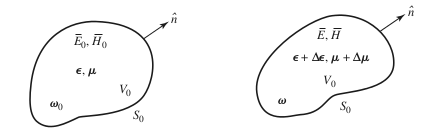
\includegraphics[scale=0.5]{perturbmaterial}
  \caption{Sistema original i sistema amb propietats pertorbades}
  \label{perturbmaterial}
\end{figure}

\begin{subequations}
  \begin{align}
    \del \times \vec E_0 &= - \jmath  \omega _0 \mu \vec H_0 \label{ori1}\\
    \del \times \vec H_0 &=  \jmath  \omega _0 \epsilon \vec E_0 \label{ori2} 
  \end{align}
\end{subequations}

I els del sistema pertorbat satisfan

\begin{subequations}
  \begin{align}
    \del \times \vec E &= - \jmath  \omega (\mu + \Delta \mu) \vec H \label{new1} \\
    \del \times \vec E &= \jmath  \omega (\epsilon + \Delta \epsilon) \vec H \label{new2}
  \end{align}
\end{subequations}

Multipliquem  \cref{ori1}$^*$ per $\vec H$ i restem $\vec E^* \cdot$ \cref{new2}

\begin{equation}
  \del (\vec E_0^* \times \vec H_0 ) = \jmath \omega_0 \mu \vec H_0^* \cdot \vec H - \jmath \omega (\epsilon + \Delta \epsilon) \vec E_0 ^* \cdot \vec E \label{eq5}
 \end{equation}

I fent $\vec E \cdot$ \cref{ori2}$^*$ - $\vec H_0 ^*$ \cref{new1}

\begin{equation}
  \del (\vec E_0 \times \vec H_0 ^*) = \jmath \omega \epsilon \vec E_0^* \cdot \vec E - \jmath \omega (\mu + \Delta \mu) \vec H_0 ^* \cdot \vec H \label{eq6}
\end{equation}

Integrem la suma de \cref{eq5,eq6}:

\begin{equation}
  \begin{aligned}
  \int _{V_0} \del ( \vec E_0 ^* \times \vec H + \vec E \times \vec H_0 ^*) dV = \int \bigg [ &\jmath ( \omega_0 - \omega) \epsilon \vec E_0 ^* \cdot \vec E + \jmath (\omega_0 - \omega) \mu \vec H_0 ^* \cdot \vec H \\
  - &\jmath \omega \Delta \epsilon \vec E _0 ^* \cdot \vec E - \jmath \omega \Delta \mu \vec H_0 ^ * \cdot \vec H \bigg ] dV
  \end{aligned}  
\end{equation}

Usem el teorema de la divergència en la primera integral

\begin{equation}
  \begin{aligned}
  \int _{S_0}  (\vec E_0 ^* \times \vec H + \vec E \times \vec H_0 ^*) \cdot \vec dS = \int \bigg [ &\jmath ( \omega_0 - \omega) \epsilon \vec E_0 ^* \cdot \vec E + \jmath (\omega_0 - \omega) \mu \vec H_0 ^* \cdot \vec H \\
  - &\jmath \omega \Delta \epsilon \vec E _0 ^* \cdot \vec E - \jmath \omega \Delta \mu \vec H_0 ^ * \cdot \vec H \bigg ] dV \label{integral}
  \end{aligned}
\end{equation}

Com que els camps elèctrics són perpendiculars a la superfície la integral sobre $S$ és zero, i manipulant els termes de la integral sobre $V$ obtenim

\begin{equation}
  \frac{\omega - \omega _0}{\omega} = \frac{\int _{V_0} \left [ \Delta \epsilon \vec E_0 ^* \cdot \vec E + \Delta \mu \vec H_0 ^* \cdot \vec H \right ] dV}{\int _{V_0} \left [ \epsilon \vec E _0 ^ * \cdot \vec E + \mu \vec H_0 ^* \cdot \vec H \right] dV}
\end{equation}

Si coneguérem $\vec E_0$, $\vec H_0$, $\vec E$ i $\vec H$ podríem calcular $\omega$ exactament. Com que no els coneguem assumirem  que $\vec E \simeq \vec E_0$ i $\vec H \simeq \vec H_0$, ja que $\Delta \epsilon$ i $\Delta \mu$ són molt xicotets.

\begin{equation}
  \frac{\omega - \omega _0}{\omega} = \frac{\int _{V_0} \left [ \Delta \epsilon \vec E_0 ^* \cdot \vec E_0 + \Delta \mu \vec H_0 ^* \cdot \vec H_0 \right ] dV}{\int _{V} \left [ \epsilon \vec E_0 ^ * \cdot \vec E_0 + \mu \vec H_0 ^* \cdot \vec H_0 \right] dV} = \frac{\Delta W}{W}
\end{equation}

La última igualtat, on $W$ és la energia emmagatzemada als camps, es deu a que les integrals són les del teorema de Poynting. Noteu que cal integrar el denominador sobre tot el volum $V_0$, però el numerador pot acotar-se a la zona pertorbada.

\subsection{Pertorbació de forma}

Si la pertorbació consisteix en un canvi en la forma, i no en els materials (figura \cref{perturbshape}), repetim el procés anterior fins a arribar a \cref{integral}, amb la diferència de que ara $\Delta \epsilon = \Delta \mu = 0$:

\begin{figure}[ht]
  \centering
  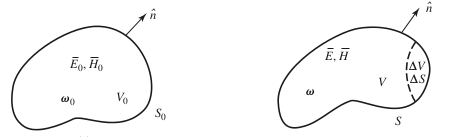
\includegraphics[scale=0.5]{perturbshape}
  \caption{Sistema original i sistema amb forma pertorbada}
  \label{perturbshape}
\end{figure}

\begin{equation}
  \int _{S_0}  (\vec E_0 ^* \times \vec H + \vec E \times \vec H_0 ^*) \cdot \vec dS = \jmath ( \omega_0 - \omega) \int \left [  \epsilon \vec E_0 ^* \cdot \vec E + \mu \vec H_0 ^* \cdot \vec H \right ] dV
\end{equation}

i podem arribar a l' expressió exacta 
\begin{equation}
  \omega - \omega_0 = \frac{- \jmath \oint _{\Delta S} \vec E_0 ^* \times \vec H_0 \vec dS}{\int _V (\epsilon \vec E_0 \cdot \vec E_0 ^* + \mu \vec H_0 \cdot \vec H_0^*) dV}
\end{equation}

On hem suposat, com abans, que $\vec E \simeq \vec E_0$ i $\vec H \simeq \vec H_0$, ja que $\Delta S \simeq 0$. També com abans podem integrar el numerador solament en la zona pertorbada.

\section{Teoria de modes acoblats}

De vegades passa que dos modes interaccionen entre ells de manera que hi ha un transvasament d' energia d' un a l' altre, com en els acobladors de senyal, en estructures periòdiques en moduladors acusto-òptics, en amplificadors... La teoria de modes acoblats ens permet obtindre el resultat d' acoblaments com aquests, i és més general: pot ser aplicada a modes no electromagnètiques, o a acoblaments entre modes EM i no EM (com acústics, o ones d' electrons).

\subsection{Acoblament de modes copropagants}

Si en una guia en la que es propaga més d' un mode de manera independent fem una pertorbació podem provocar que els modes deixen de ser independents. Suposem que el mode resultant és una combinació lineal dels modes originals 1 i 2:

\begin{subequations}
  \begin{align}
    \vec E ' &= A_1(z) \vec E_1 e^{-\jmath \beta_1 z} + A_2 (z) \vec E_2 e^{-\jmath \beta _2 z } \\
    \vec H ' &= A_1 (z) \vec H_1 e^{-\jmath \beta _1 z} + A_2 (z) \vec H_2 e^{-\jmath \beta_2 z}
  \end{align}
\end{subequations}

i intentem trobar $A_1(z)$ i $A_2(z)$. Per un procediment similar al de la secció anterior arribem a la igualtat

\begin{equation}
  \del \left [ A_1(z) (\vec E_1^* \times \vec H_1 + \vec E_1 \times \vec H_1 ^ * ) + A_2 (z) (\vec E_1 ^* \times \vec H_2 +  \vec E_2 \times \vec H_1 ^* ) \right ] = - \jmath \omega \Delta \epsilon  \vec E_1 ^* \cdot \vec E \label{igualtat}
\end{equation}

Integrem ambdós costats sobre la secció transversal $S_t$ i apliquem el teorema de la divergència en 2 dimensions. Anomenant $\vec F$ a la suma dins del $\del$ en \cref{igualtat} arribem a

\begin{equation}
  \pd{}{z} \int_{S_t} \vec F \cdot \vec dS + \oint _{C(S_t)} \vec F \cdot \vec n dl = - \jmath \omega \Delta \epsilon \int _{S_t} \vec E_1 ^* \cdot \vec E dS
\end{equation}

En cas de que les parets siguen conductores la integral de contorn desapareixerà, ja que $\vec E \times \vec H$ és tangent a aquestes. Si són dielèctriques el integrant és proporcional a $\frac{1}{r}$, i considerant contorns infinits deduïm que ha d' anul·lar-se igualment.

Si reescrivim $\vec F$ explícitament i calculem la derivada sobre la integral arribem a:

\begin{equation}
  \begin{aligned}
  \pd{A_1}{z} &= -\jmath \omega \int \left[ \Delta \epsilon \vec E_1 ^* e^{-\jmath \beta _1 z} ( A_1 e^{\jmath \beta _1 z} \vec E_1 + A_2 e^{\jmath \beta _2 z} \vec E_2) \right] dS \\
  &= k_{11} A_1 (z) + k_{12} A_2(z) e^{\jmath \delta z}
  \end{aligned}
\end{equation}

On hem definit 

\begin{subequations}
  \begin{align}
    \delta &= \beta_2 - \beta_1 \nonumber \\
    k_{11} &= -\jmath \omega \int \Delta \epsilon \abs{\vec E_1} ^2 dS \nonumber \\
    k_{12}& = -\jmath \omega \int \Delta \epsilon \vec E_1 ^* \cdot \vec E_2 dS \nonumber \\
  \end{align}
\end{subequations}

I, similarment,

\begin{equation}
  \pd{A_2}{z} = k_{22} A_2 (z) + k_{21} A_1(z) e^{\jmath \delta z}
\end{equation}

amb

\begin{subequations}
  \begin{align}
    k_{22} &= -\jmath \omega \int \Delta \epsilon \abs{\vec E_2} ^2 dS \nonumber \\
    k_{12} &= k_{21}^* \nonumber \\
  \end{align}
\end{subequations}

D' aquestes dues equacions podem calcular $A_1$, i $A_2$ en funció de $\delta$ i $\epsilon$. En general observarem que les seues amplituds $\abs{A_1}^2$ i $\abs{A_2} ^2$ estan en contrafase, ja que l' energia que un dels modes perd el guanya l' altre.